\chapter{Experiments with Artificial Neural Tensors} 
\label{chapter-artifical} 
We generated the neural manifold for artificial neural networks (ANNs) using the same approach as we did for biological neural networks in the previous chapter. But unlike the latter where the neural tensors were already available from the lab experiments, we need to first build the artificial neural tensor by taking the outputs of neuron units in pre-trained ANNs. 

\section{Building the artificial neural tensor}
In the first semester, we have been focusing on investigating the manifold structure of CNN, and specifically the VGG-16 model, but the same method applies to any ANNs. VGG-16 is one of the most successful CNN models in computer vision tasks such as image classification. Its architecture is shown in the figure below. Since previous works have already trained the VGG-16 model to obtain optimal weights, we will directly use the pre-trained weights to generate the artificial neural tensor. 

\begin{figure}[H]
        \centering
            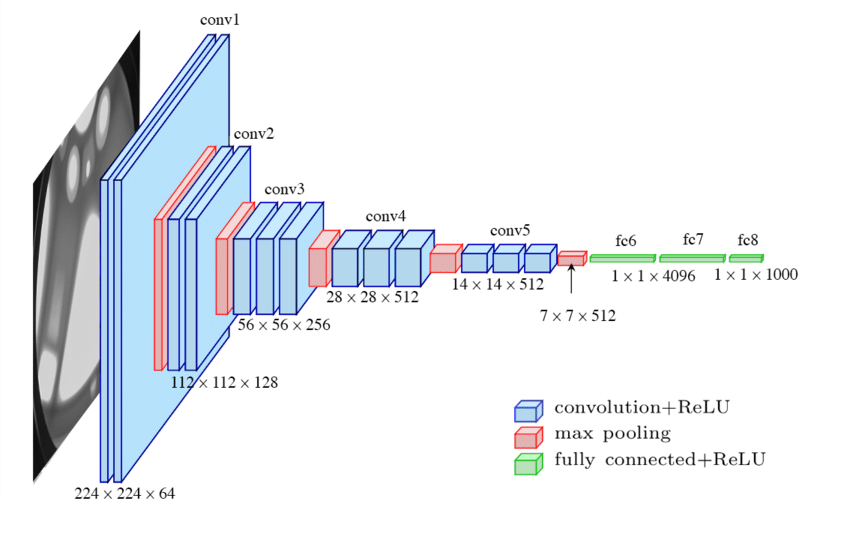
\includegraphics[width=0.9\textwidth]{figures/artificial/vgg16.png}
            \caption{Visualizing the structure of the VGG-16 model.}
    \end{figure}
    
\subsection{``Visual stimuli" in ANNs}
Analogous to the visual flows used in lab experiments, the ``visual stimuli" for ANNs are natural images of different objects (e.g. cars, cats, and dogs) selected from the commonly used data set, CIFAR-10 (\cite{Krizhevsky09cifar-10}). CIFAR-10 consists of 60000 32x32 colour images in 10 classes, with 6000 images per class. To keep the size of the artificial neural tensor manageable, we randomly selected 10 images from each class as the visual stimuli. In order to simulate the movement of visual flows used in lab experiments, we implemented the shifts in image, that is, for every image we shifted the image vertically and horizontally (by one pixel per step). 
    % add image
    \begin{figure}[H]
        \centering
            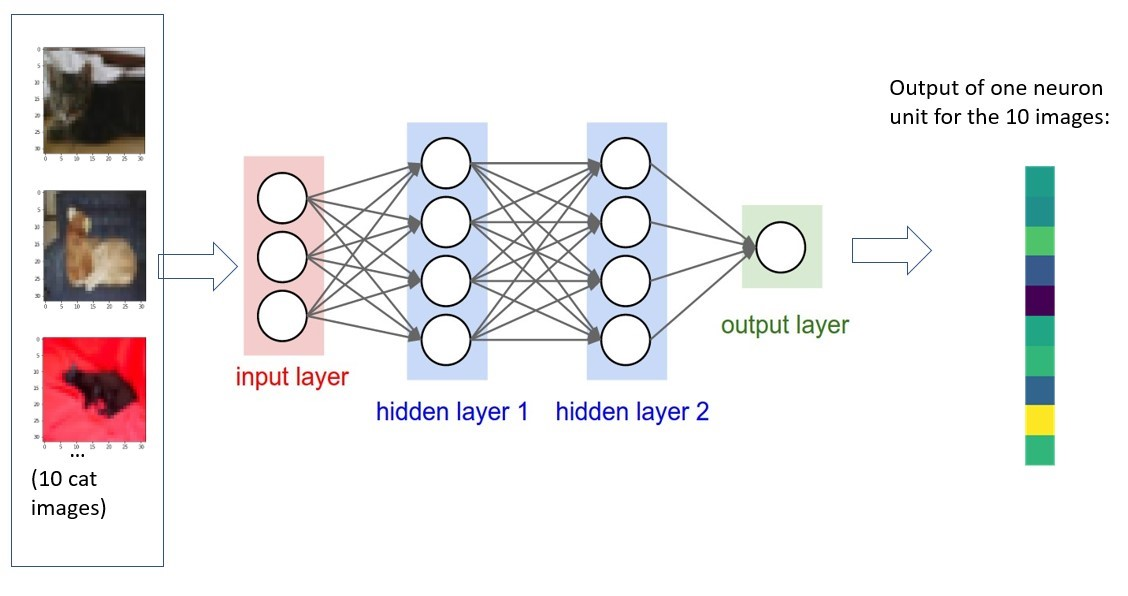
\includegraphics[width=0.9\textwidth]{presentation/Slide1.jpg}
            \caption{Computing output of one neuron unit in the ANNs given 10 input cat images.}
    \end{figure}

\begin{rmk}
At first it might seem that the use of different ``visual stimuli" for biological and artificial neural networks will lead to an unfair comparison. However, this approach is appropriate for the following reason. The mouse visual system was trained on naturalistic visual information and the visual flows used in the lab experiments are also naturalistic. The VGG-16 model was trained on ImageNet, which are very similar to the CIFAR-10 data set that we used for ``visual stimuli" for ANNs. Thus, in both cases, the visual stimuli are similar to what the respective network was trained to recognize.

That being said, we could also adapt the experiments for ANNs to take the same visual flows as the input. In fact, it is on the agenda for the next steps in our project.
\end{rmk}
 
 \subsection{``Individual neuron'' in ANNs}
 In the lab experiments for biological neural networks, moving visual stimuli trigger spikes in the activation potential in the neurons in the retina. The individual neuron response is the firing rate of the neuron which is dependent on the  electrostatics processes that take place in the synapse. The biological neuron is coarsely modeled by the neuron unit in the ANNs. At the ``dendrite," the input is taken from the ``axons" of the connected neurons. The weight of each neuron models the synaptic process in biological neuron. At the ``cell body," all the inputs are multiplied with the weights and summed. We then add the bias term to the sum and apply the non-linear activation function to obtain the final output from this individual neuron unit at the ``axon." The parallel between an individual biological and artificial neuron is shown in the figures below. 
 
 Note that in our experiments, instead of taking the input from previously connected neuron unit, we make a modification by making each neuron unit always take the image vector as the input.
 
  \begin{figure}[H]
        \centering
            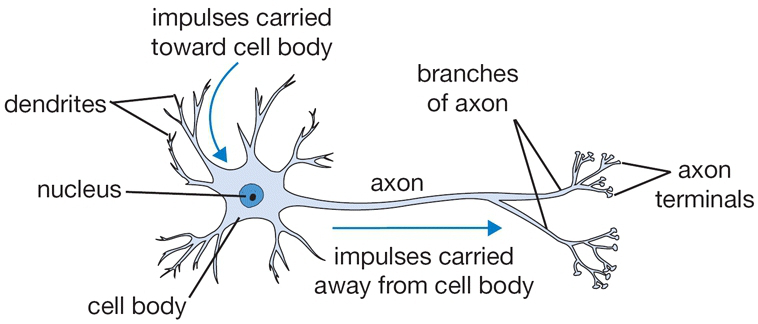
\includegraphics[width=0.9\textwidth]{figures/artificial/neuron.png}
            \caption{An individual neuron in biological neural networks. Adapted from (\cite{cs231n}).}
    \end{figure}
     \begin{figure}[H]
        \centering
            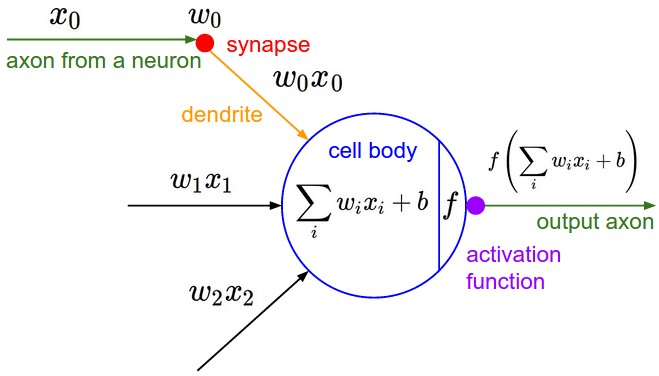
\includegraphics[width=0.9\textwidth]{figures/artificial/neuron_model.jpeg}
            \caption{An ``individual neuron" in ANNs. Adapted from (\cite{cs231n}).}
    \end{figure}
    
\subsection{``Receptive field" of an artificial neuron}
Each layer in the CNN has several different feature maps. Each feature map corresponds to a filter of a specific size and specific weights. The filter is essentially a matrix that, when taking inner product with the input image, give an output that highlights some specific features in the input image. To illustrate this, we can visualize the 64 feature maps in the first convolutional layer of the VGG-16 model, given the input bird image.
\begin{figure}[H]
        \centering
            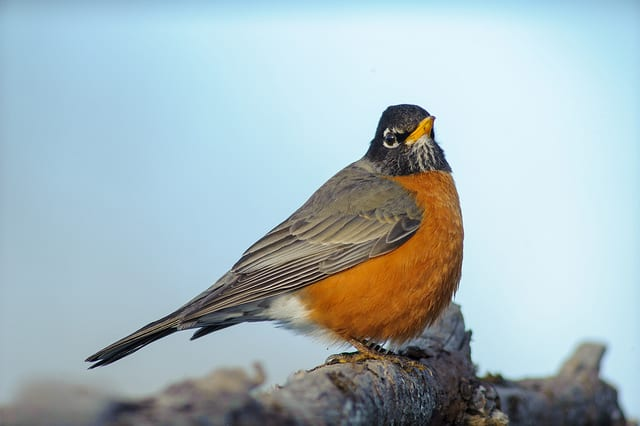
\includegraphics[width=0.9\textwidth]{figures/artificial/bird.jpg}
            \caption{Input image. Adapted from (\cite{feature_map}).}
    \end{figure}
\begin{figure}[H]
        \centering
            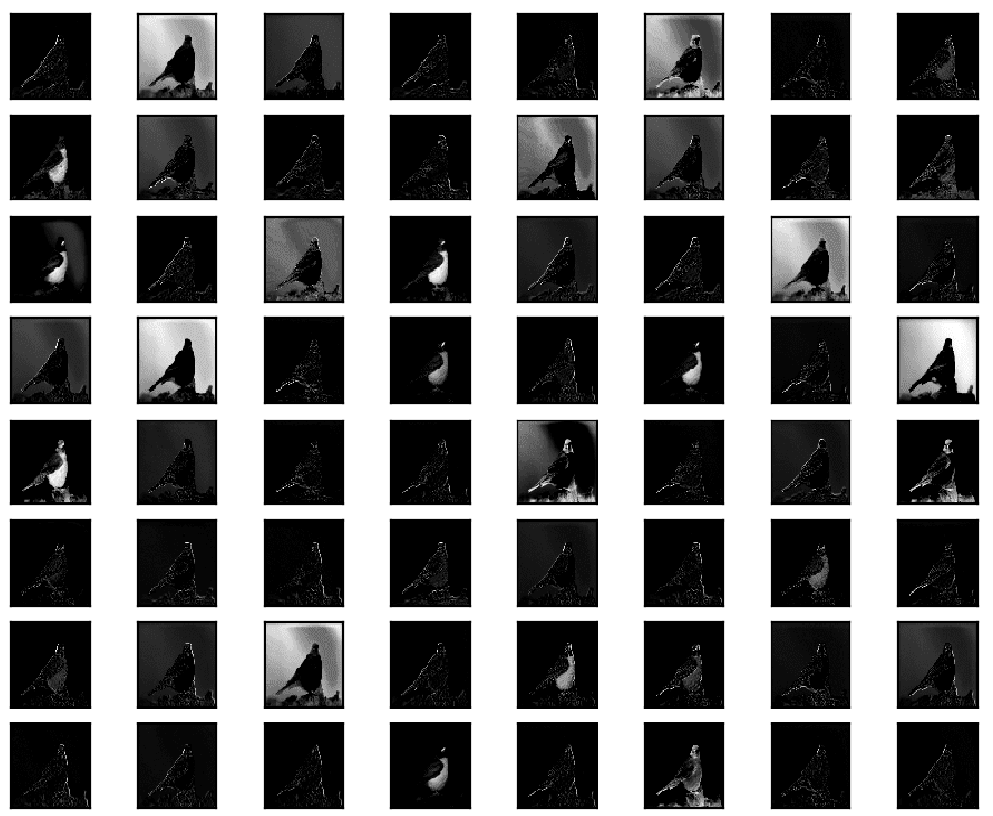
\includegraphics[width=0.9\textwidth]{figures/artificial/feature_map_vgg16.png}
            \caption{Visualizing the 64 feature maps in the first convolutional layer of the VGG-16 model. Adapted from (\cite{feature_map}).}
    \end{figure}
    
Each feature map will have a number of neurons. Each neuron attends to a specific subregion of the image, which is called their ``receptive field." This term in fact originated from the study of the biological visual system, which is defined as a restricted region of visual space where a luminous stimulus could drive electrical responses in a retinal ganglion cell.

The size of the receptive field of is the same as the filter size corresponding to the feature map in which the neuron is located. Each neuron will have the same set of weights as the other neurons in the same feature map (this is sometimes called ``weights sharing"). 

 \subsection{``Neuron population response" in ANNs}
Analogous to the neuron population response in biological neural networks, we computed the all the neuron output given the input image and analyze them collectively, instead of looking at each neuron output individually.

However, one difference from the biological neural networks is that given an image input, most of the neurons will have output of small values (since except for the specific neurons that target at recognizing a specific features, a large number of pre-trained weights are close to zero). In other words, the ``firing" of neurons in ANNs will be sparse. Thus, we selected only ten feature maps with highest average firing rate (the average is taken over all neurons in the respective feature map). 

We now illustrate the dimensions of the resulting artificial neural tensor built from the first convolutional layer of VGG-6. Since there were 1024 neurons in each feature map and we selected 10 feature maps, there were 10240 neurons in total. The visual stimuli consists of 10 images from each of the 10 classes, which give us 100 images. Each of the images have 1024 shifts. In the end, the size of the artificial tensor for the first convolutional layer is thus 10240-by-100-by-1024. 

\section{Applying tensor CP decomposition}
Having built the artificial neural tensor, we then applied the tensor CP decomposition to obtain the first five tensor factors: 
      \begin{figure}[H]
        \centering
            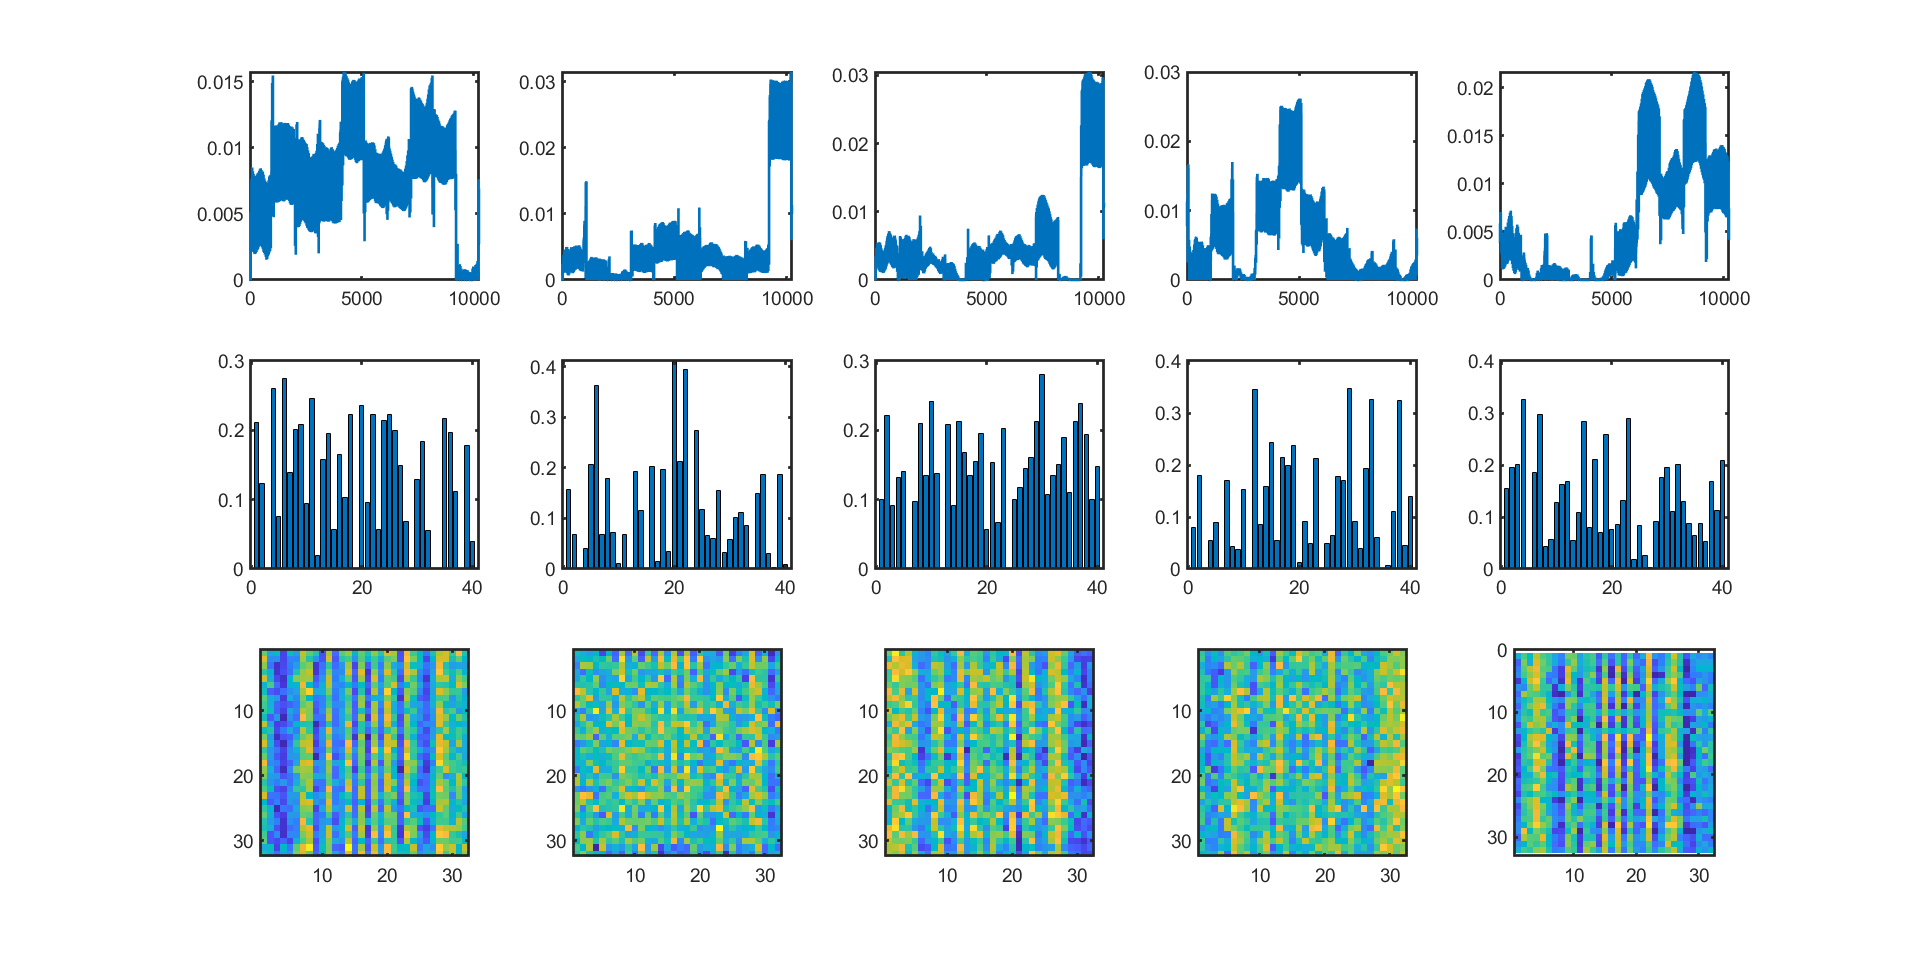
\includegraphics[width=\textwidth]{artificial-tensor/results/nonneg_factors_3D.png}
            \caption{First 5 tensor factors for artificial neural data.}
        \end{figure} 

We then generated the neural manifolds from artificial neural tensor, which can be visualized in the following plot. 
    \begin{figure}[H]
        \centering
            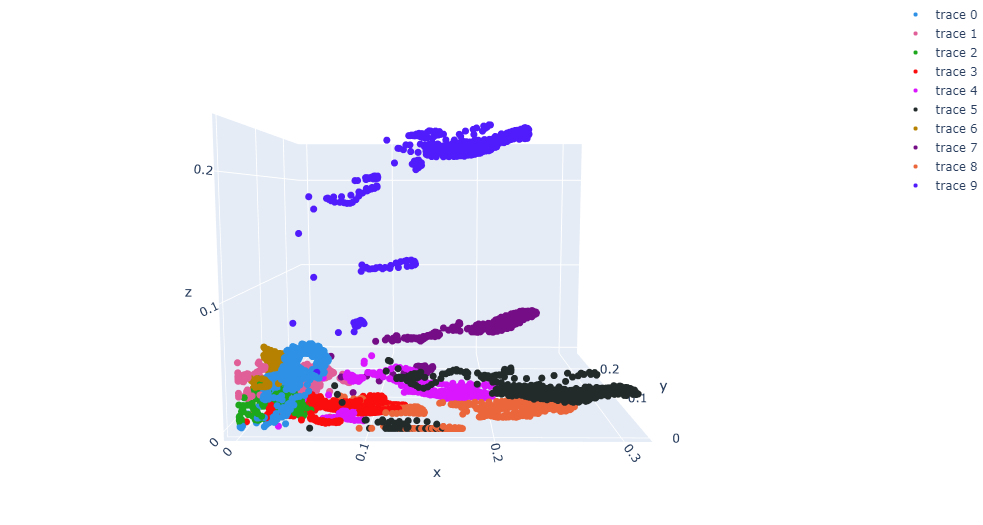
\includegraphics[width=\textwidth]{artificial-tensor/results/TCA_3D.png}
            \caption{Neural manifold generated from artificial neural tensor.}
        \end{figure} 
